\section{Differentials, coordinate transformations, 
unisolvence and conformity of Finite Elements}

For \noindent{\color{BrickRed} SOME of}  the following exposition we refer to~\cite{ciarlet},
 Section 3.9 of~\cite{monk} and~\cite{gh99}.

We want this same setting to build Finite Elements on 
arbitrary contiguous prisms
belonging to a fixed mesh, all of which being an affine 
image of the reference prism.
In order to do so we transform the set $\hat{E}$ and show how to
pull--back and forward the scalars and fields in the 
discrete local spaces and the corresponding 
degrees of freedom.

%===============
%exactly as we are told by the 
%push-forward
%transformations~(\ref{push-forward}). 
%===============

Consider the application $\hat{\bx}\longmapsto{\bx} = 
F_E(\hat{\bx})$, where 
\begin{IEEEeqnarray}{rCl} \label{aux_label8}       
  F_E &= &M_E\hat{\bx} + \bx_0\mbox{, } 
\end{IEEEeqnarray}
that transforms
$\hat{E}$ in an element $E$ of the mesh and $M_E$ is invertible.

A scalar function $\hat{p} \in H^1(\hat{E})$ is transformed into a 
scalar function $p$ on $E$ with
\begin{IEEEeqnarray}{rCl}
    \label{transfEscalar} p\circ F_E & = & \hat{p}.
\end{IEEEeqnarray}
As it holds~(\cite{ciarlet})
\begin{IEEEeqnarray}{rCl} \label{aux_label4}
  \nabla p = M^{-t}\hat{\nabla} \hat{p} \circ F_K^{-1}\mbox{,}
\end{IEEEeqnarray}
then it results 
$p \in H^1(K)$. Gradients are taken with respect to the local coordinates
of $E$ and $\hat{E}$ in each case. The same will apply for every finite element
and for $\dv$ and $\curl$.

Now let $\hat{\bu} \in H(\bcurl, \hat{E})$. We want to assign to it a function
$\bu$ on $E$. As for $\hat{p}$ and $p$ as before it holds
$\nabla p \in H(\bcurl, E)$ and $\hat{\nabla} \hat{p} \in H(\bcurl, \hat{E})$,
equality~(\ref{aux_label4}) suggests the following transformation.
\begin{IEEEeqnarray}{rCl}
    \label{transfHcurl} \bu\circ F_E & = & M_E^{-t}\hat{\bu}.
\end{IEEEeqnarray} 
With this definition we have $\bu\in H(\bcurl, E)$ and also
\begin{IEEEeqnarray}{rCl}
    \label{transfCurl} (\textbf{curl}\,\bu)\circ F_E & = & 
    \frac{1}{\det M_E} M_E (\curl\hat{\bu})\mbox{,}
\end{IEEEeqnarray}
(cfr. Lemma 3.57, page 77 and Corollary 3.58 in~\cite{monk}).
Now we proceed in a similar way for $H(\dv)$. The relation 
$\hat\bu\in H(\curl,\hat E)$ implies $\curl\hat\bu\in H(\dv, \hat E)$
so~(\ref{transfCurl}) shows that to transform $\hat\bu\in H(\dv,\hat E)$
into $\bu\in H(\dv,E)$ we must do it via
\begin{IEEEeqnarray}{rCl}\label{transfDiv}
	\bu\circ F_E & = & \frac{1}{\det M_E}M_E\hat\bu.
\end{IEEEeqnarray}
If $\bu$ and $\hat\bu$ are related
by~(\ref{transfDiv}), then with a $\mathcal{D}(E)$ density argument we get 
\begin{IEEEeqnarray}{rCl} %% By Lemma 3.59 in~\cite{monk}
  \label{derivadaPiola} (\dv\,\bu)\circ F_E & = & (\det M_E)^{-1}\dv\,\hat\bu.
\end{IEEEeqnarray}
and hence $\bu\in H(\dv,E)$ if and only if $\hat\bu\in H(\dv,\hat E)$.

Normals and tangents are transformed as follows (cfr. page 265 of~\cite{giraultRaviart}).
Let $\hat{\bnu}$ be the unit outward normal to $\hat E$
If $\hat\bx\in\partial \hat{E}$ and $\bnu$ is defined by
\begin{IEEEeqnarray}{rCl} \label{aux_label9}
  \bnu(F_E\hat\bx)&=&
    \frac{M_E^{-t}\hat{\bnu}(\hat\bx)}{\|M_E^{-t}\hat{\bnu}(\hat\bx)\|}\mbox{,}
\end{IEEEeqnarray} 
then $\bnu$ is a unit normal to $E$. Second, let $\hat\btau$ be any
unit vector tangent to $\partial{\hat{E}}$ at $\hat\bx$. If $\btau$ is
given by
\begin{IEEEeqnarray}{rCl} \label{aux_label10}
  \btau(F_E\hat\bx)&=&
    \frac{M_E\hat{\btau}(\hat\bx)}{\|M_E\hat{\btau}(\hat\bx)\|}\mbox{,}
\end{IEEEeqnarray}
then $\btau$ is a unit vector tangent to $\partial E$ at $F_E\hat\bx$.
Surface differentials are changed in the following way.
\begin{IEEEeqnarray}{rCl} \label{surface_diffs}
    dS & = & \|M_E^{-t}\hat\bnu\|\,|\det B|\,d\hat{S}
\end{IEEEeqnarray}
%======================================================================
% With~(\ref{transfDiv})
% \begin{IEEEeqnarray*}{rCl}
%    \|\hat{\textbf{v}}\|^2_{L^2(\hat{E})}
%    &=& \sum_{1\leqslant i\leqslant 3}\|\hat{v}_i\|^2_{0,\hat{E}}\\[7pt]
%    &=& \sum_{1\leqslant i\leqslant 3}\frac{h_jh_k}{h_i}\,\|v_i\|^2_{0,K};\\[7pt]
%    \|\hat{v}_i\|^2_{0,\hat{E}}&=&\frac{h_jh_k}{h_i}\,\|v_i\|^2_{0,K}
% \end{IEEEeqnarray*}
% where $\{i,j,k\} = \{1,2,3\}$.
%======================================================================
%=================================================================
%\begin{lemma} For all $\tilde{\boldsymbol{\sigma}} \in H(\dvg, \tilde{K})$,
%$\boldsymbol{\sigma}$ results in
%$H(\dvg, K)$ and in fact
%\[
%    {div}\,\boldsymbol{\sigma}({\bx}) =
%        \frac{1}{\det DF}\,\tilde{{div}}\,\tilde{\boldsymbol{\sigma}}(\tilde{{\bx}}).
%\]
%\end{lemma}
%\begin{proof}
%Observe that
%\begin{IEEEeqnarray*}{rCl}
%    trace(A\cdot B\cdot A^{-1}) &=& trace(B)\\
%    \label{Piola}\yesnumber\boldsymbol{\sigma} \circ F & = & \frac{1}{\det(A)} A\,\tilde{\boldsymbol{\sigma}}\\
%    \label{derivadaPiola}\yesnumber D\tilde{\boldsymbol{\sigma}}(\tilde{\bx}) & = &
%        \det(A)\,A^{-1}\,D\boldsymbol{\sigma} (F(\tilde{\bx})) \,A.
%\end{IEEEeqnarray*}
%Then
%\begin{IEEEeqnarray*}{rCl}
%    \text{div}\,\boldsymbol{\sigma}(\bx) & = & trace(D\boldsymbol{\sigma} (\bx))\\
%                                        & = & \frac{1}{\det(A)}\,trace(A\,\tilde{D}\tilde{\boldsymbol{\sigma}} (F^{-1}(\bx))\,A^{-1})\\
%                                        & = & \frac{1}{\det(A)}\,\tilde{\text{div}}\,\tilde{\boldsymbol{\sigma}}(\tilde{\bx}).   
%\end{IEEEeqnarray*}
%\end{proof}
%=================================================================

First a key result that establishes a relation between the interpolation
operators. It will used as an important step in the proof of the stability of the
edge element as well as in the proof of the stability of the face elements.
\begin{remark} Lemma 5.40 in page 135 and the first Paragraph of Section 5.7 
in page 149 of~\cite{monk} state the following facts.
  
Take $\bw_E$ es el operador de interpolaci\'on determinado por el elemento en
la Definici\'on~\ref{edgeelement}, $\br_E$ es el operador de interpolaci\'on determinado por el elemento en la
Definici\'on~(\ref{defi_h_div_conforme}) and $\pi^{\perp}_E$ is
the $L^2$--orthogonal projection onto $P_k(E)$, then 
\begin{enumerate}
  \item 
For all sufficiently smooth $\bu$ such that both the interpolants
$\bw_E\bu$ and $\br_E\curl\bu$ are defined, then
\begin{IEEEeqnarray}{rCl}
\label{curl_commutativity}
  \curl\bw_E\bu &=& \br_E\curl\bu.
\end{IEEEeqnarray}
  \item 
For all sufficiently smooth $\bu$ such that both the interpolants
$\br_E\bu$ and $\pi^{\perp}_E\dv\bu$ are defined, then
\begin{IEEEeqnarray}{rCl}
\label{div_commutativity}
  \dv\,\br_E\bu & = & \pi^{\perp}_E\dv\,\bu.
\end{IEEEeqnarray}
\end{enumerate}
\end{remark}
%=============================================================
% \begin{proof}
% Vamos a usar la siguiente versión superficial del Teorema de Stokes. Sea dado un dominio Lipschitz acotado 
% $S\subseteq\mathbb{R}^2$ con tangente unitaria $\boldsymbol{\tau}$ al borde $\partial S$. Para 
% $\bu \in \mathcal{C}^1(\bar{S})^2 $ y $\phi \in \mathcal{C}^1(\bar{S})$ tenemos
% \begin{IEEEeqnarray}{rCl}
%     \int\limits_S \bu d\gamma & = &   %% HACER SEGUIR ACA
% \end{IEEEeqnarray}
% \end{proof}
%=============================================================
\noindent The last result can be expressed saying that the following diagram commutes:
\begin{center}
        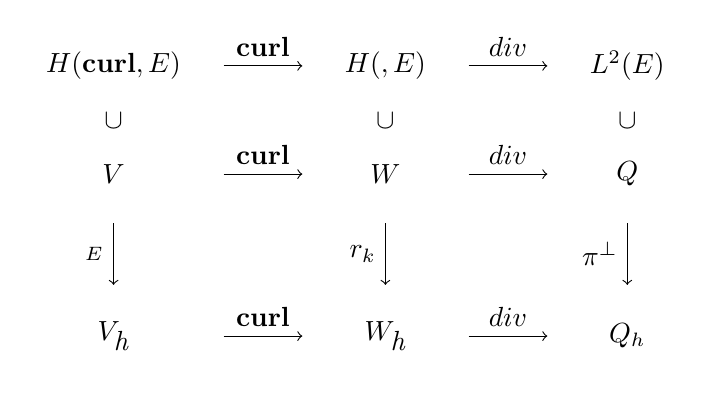
\begin{tikzpicture}[point/.style={circle, inner sep=0pt, minimum size=2pt,fill=red}]
            \matrix[column sep = 1.82mm, row sep = 1.1mm, ampersand replacement = \&] {
             \node {$\text{H}(\textbf{curl},E)$};  
              \& \node (n0) {};
              \& \node      {};
              \& \node (n1) {};
              \& \node (n2) {};
              \& \node {$\text{H}(\Div, E)$}; 
              \& \node (r1c7) {};
              \& \node {};
              \& \node {};
              \& \node (r1c10) {};
              \& \node {$L^2(E)$};\\
             \node (n3) {}; \&\&\&\&\& \node (n5)   {};
              \& \node (r2c7) {};
              \& \node {};
              \& \node {};
              \& \node {};
              \& \node (r2c11) {};\\
             \node (n4) {}; \&\&\&\&\& \node (n6)   {};
              \& \node (r3c7) {};
              \& \node {};
              \& \node {};
              \& \node {};
              \& \node (r3c11) {};\\
             \node (v)  {$V$}; \&\node(fromV){};\&\&\&\node(toW){};\& \node (w) {$W$};
              \& \node (r4c7) {};
              \& \node {};
              \& \node {};
              \& \node (r4c10) {};
              \& \node {$Q$};\\
             \node (n7) {}; \&\&\&\&\& \node (n8)   {};
              \& \node {};
              \& \node {};
              \& \node {};
              \& \node {};
              \& \node (r5c11) {};\\
             \node      {}; \&\&\&\&\& \node        {}; 
              \& \node {};
              \& \node {};
              \& \node {};
              \& \node {};
              \& \node {};\\
             \node      {}; \&\&\&\&\& \node        {}; 
              \& \node {};
              \& \node {};
              \& \node {};
              \& \node {};
              \& \node {};\\
             \node (n11)    {}; \&\&\&\&\& \node (n12) {};
              \& \node {};
              \& \node {};
              \& \node {};
              \& \node {};
              \& \node (r8c11) {};\\
             \node {$V_{\textit{h}} $};                                 
              \& \node (n13) {};
              \& \node       {};
              \& \node (n14) {};
              \& \node (n15) {};
              \& \node {$W_{\textit{h}} $}; 
              \& \node (r9c7) {};
              \& \node {};
              \& \node {};
              \& \node (r9c10) {};
              \& \node {$Q_h$};\\
             };
            \draw[->] (n0) to node[above] {$\textbf{curl}$} (n2); 
            \draw[->] (fromV) to node[above] {$\textbf{curl}$} (toW); 
            \draw[white] (n3) to node {{\color{black}$\cup$}} (n4);
            \draw[white] (n5) to node {{\color{black}$\cup$}} (n6);
            \draw[->] (n7) to node[left] {$\bw_E$} (n11); 
            \draw[->] (n8) to node[left] {$\boldsymbol{r}_k$} (n12); 
            \draw[->] (n13) to node[above] {$\textbf{curl}$} (n15); 
            \draw[->] (r1c7) to node[above] {$\text{div}$} (r1c10);
            \draw[->] (r4c7) to node[above] {$\text{div}$} (r4c10);
            \draw[->] (r9c7) to node[above] {$\text{div}$} (r9c10);
            %\draw[white] (r2c7) to node {{\color{black}$\cup$}} (r3c7);
            \draw[white] (r2c11) to node {{\color{black}$\cup$}} (r3c11);
            \draw[->] (r5c11) to node[left] {$\pi^{\perp}$} (r8c11);
        \end{tikzpicture}
    \end{center}
\begin{equation}\label{push-forward}
  \mbox{\color{red} \ldots \mbox{push-forward} de los interpoladores\\
    y que los pull--backs conmutan con los interpoladores}
\end{equation}
{\bf hcurl}
  
\begin{lemma} \label{aux_label7}
Let $\hat E$ be the reference prism~(\ref{defi_of_ref_prism}) and
let $P_{\hat E}$ be the space in~(\ref{spaceFEprismHcurl}), that is,
\begin{IEEEeqnarray*}{rCl}
  P_{\hat{E}} & = & R_k(\hat{x}_1,\hat{x}_2) \otimes P_k(\hat{x}_3) \times 
            P_k(\hat{x}_1,\hat{x}_2) \otimes P_{k-1}(\hat{x}_3).
\end{IEEEeqnarray*}
Provided the matrix $M_E$ is block--diagonal in this manner
\begin{IEEEeqnarray*}{rCl}
  M_E & = & \blockdiag{m_{1,1}}{m_{1,2}}{m_{2,1}}{m_{2,2}}{m_{3,3}}\mbox{,}
\end{IEEEeqnarray*}
then $P_{\hat{E}}$ is invariant by transformation~(\ref{transfHcurl}).
\end{lemma}
\begin{proof}
  Starting with transformation~(\ref{transfHcurl}) take 
  $\hat{\bu}=(\hat u_1,\hat u_2,\hat u_3)'\in P_{\hat E}$
  and $\bu := (M_E^{-t}\hat{\bu})\circ F_E^{-1}$.
  Let 
  \[
    M_2 = \left(
    \begin{array}{cc}
      m_{1,1}  & m_{1,2}\\
      m_{2,1}  & m_{2,2} 
    \end{array}
    \right)
  \]
  and let $m_{i,j}^{(-1)}$ denote the coefficients of the inverse.
  By definition, 
  $(\hat u_1,\hat u_2)' = \hat{q}(\hat\bp + \hat{\boldsymbol{s}})$ for some
  $\hat\bp$, $\hat{\boldsymbol{s}}$ as in~(\ref{defSk}) and~(\ref{defRk}) and
  $\hat{q}\in P_{k}(\hat x_3).$ Using the blocks of $M_E$ and the tensor nature of
  $P_{\hat E}$,
  \begin{IEEEeqnarray*}{rCl}
    (\hat u_1(\bx),\hat u_2(\bx))' & = & (\hat{q}M_2^{-t}(\hat\bp + 
      \hat{\boldsymbol{s}}))(M_E^{-1}\bx - M_E^{-1}\bx_E)\\
    & = & \hat{q}(m_{3,3}^{(-1)}(x_3-x_{E,3}))(M_2^{-t}(\hat\bp + 
      \hat{\boldsymbol{s}}))(M_2^{-1}\bx - M_2^{-1}\bx_E).
  \end{IEEEeqnarray*}
  Now, $\hat{q}(m_{3,3}^{(-1)}(x_3-x_{E,3}))$ is a polynomial $q(x_3)$ with the
  same 
  degree as $\hat{q}$ is qith respect to $\hat x_3$. Furthermore,
  as by Remark~(\ref{aux_label6}) $\hat{\boldsymbol{s}}$ has degree $\leqslant k-1$,
  $(M_2^{-t}(\hat\bp + \hat{\boldsymbol{s}}))(M_2^{-1}\bx - M_2^{-1}\bx_E)$
  can be seen as
  $M_2^{-t}(\bp(x_1,x_2) + \hat{\boldsymbol{s}}(M_2^{-1}\bx))$ with $\bp$
  having the expected degrees. And now
  \begin{IEEEeqnarray*}{rCcCl}
    M_2^{-t}\hat{\boldsymbol{s}}(M_2^{-1}\bx)\cdot(x_1,x_2)'
        &=& 
    \hat{\boldsymbol{s}}(M_2^{-1}(x_1,x_2)')\cdot M_2^{-1}(x_1,x_2)' &=& 0.
  \end{IEEEeqnarray*}
  The invariance of the third component of elements in $P_{\hat E}$ is
  an immediate consequence of the affine nature of the coordinate change.
\end{proof}
%=======================================================================
%\begin{remark} this is not a restriccion...
%  \begin{figure}
%    \centering
%    *** ***
%    \caption{hybrid mesh}\label{obliquePrism}
%  \end{figure}
%  dibujo prisma oblicuo subdividido: tetra + prism + pyramid. Figure~\ref{obliquePrism}
%\end{remark}
%=======================================================================
\begin{lemma} Let a physical prism $E = F_E(\hat{E})$ for $F_E$ as in~(\ref{aux_label8}).
Given $\hat\bu$ defined in $\hat{E}$ let $\bu$ in $E$ dtermined by~(\ref{transfHcurl}), and
let $\hat\btau$, $\btau$, $\hat\bnu$ and $\bnu$ be tangents and normals in
$\hat E$ and $E$ related by~(\ref{aux_label10}) and~(\ref{aux_label9}). Suppose
we define degrees of freedom of $\bu$ on $E$ as
\begin{IEEEeqnarray}{ll}
    \label{momentos1hcurlPhys}  
    \varphi_{\hat{\be}_i,p}\,(\bu) **= 
    \int_{\be} \bu \cdot \boldsymbol{\tau} \,q\, ds  
        & q\in P_{k-1}\mbox{,} \\
    \IEEEeqnarraymulticol{2}{l}{\nonumber\mbox{ for each edge $\be$ with unit tangent } \boldsymbol{\tau} \mbox{;}}\\[8pt]
    \label{momentos2hcurlPhys} 
    \varphi_{f_j,\bq}\,(\bu) **=  
    \int\limits_{f} \textbf{u} \times \bnu \cdot \bq\,
    d\gamma\mbox{, } &\bq = (q_1,q_2,0) \in P_{k-2}^2 \times \{ 0 \},\\ 
    \IEEEeqnarraymulticol{2}{l}{\nonumber\mbox{ for each horizontal face $f$ with normal } \bnu = (0,0,\pm1) \mbox{;}}\\[8pt]
    \label{momentos3hcurlPhys}
    \varphi_{f_j,\bq}\,(\bu) **=  
    \int\limits_{f} \textbf{u} \times \bnu \cdot \bq\,
    d\gamma\mbox{, } &\bq = (0,q_3,q_2) \in \{ 0 \} \times Q_{k-2,k-1} \times 
    Q_{k-1,k-2}\mbox{, } \\
    \IEEEeqnarraymulticol{2}{l}{\nonumber\mbox{ for the face } f \subseteq \{ x=0 \} \mbox{ with normal }\bnu = (-1,0,0) \mbox{;}}\\[8pt]
    \label{momentos4hcurlPhys}
    \varphi_{f_j,\bq}\,(\bu) **=  
    \int\limits_{f} \textbf{u} \times \boldsymbol{n} \cdot \bq\,
    d\gamma\mbox{, } & \bq = (q_3,0,q_1) \in Q_{k-2,k-1} \times \{ 0 \} \times
    Q_{k-1,k-2},\\
    \IEEEeqnarraymulticol{2}{l}{\nonumber\mbox{ for the face } f \subseteq \{ y=0 \} \mbox{ with normal }\boldsymbol{n} = (0,-1,0) \mbox{;}}\\[8pt]
    \label{momentos5hcurlPhys}
    \varphi_{f_j,\bq}\,(\bu) **=  
    \int\limits_{f} \textbf{u} \times \boldsymbol{n} \cdot \bq\,
    d\gamma\mbox{, } & \bq = (0,q_3,q_1) \in \{ 0 \} \times Q_{k-2,k-1} \times
    Q_{k-1,k-2}\mbox{, }\\
    \IEEEeqnarraymulticol{2}{l}{\nonumber\mbox{ for the face }f \subseteq \{x+y=1\} \mbox{ with normal }\boldsymbol{n} = (1,1,0) \mbox{;}}\\[8pt]
    \label{momentos6hcurlPhys}
    \varphi_{\br}(\bu) = 
    \int_{E} \bu \cdot \br \, d\bx\mbox{, }&\br = (\det M_E)^{-1} M_E\hat\br \circ F_E^{-1}\\
    &{\nonumber\hat\br \in P_{k-2,k-2} \times P_{k-3,k-1}.}
\end{IEEEeqnarray}
Provided $\det > 0$, the degrees of freedom are identical
\end{lemma}
\begin{proof}
  Edge dofs: ver foto
  \begin{figure}[!h]
    \centering
    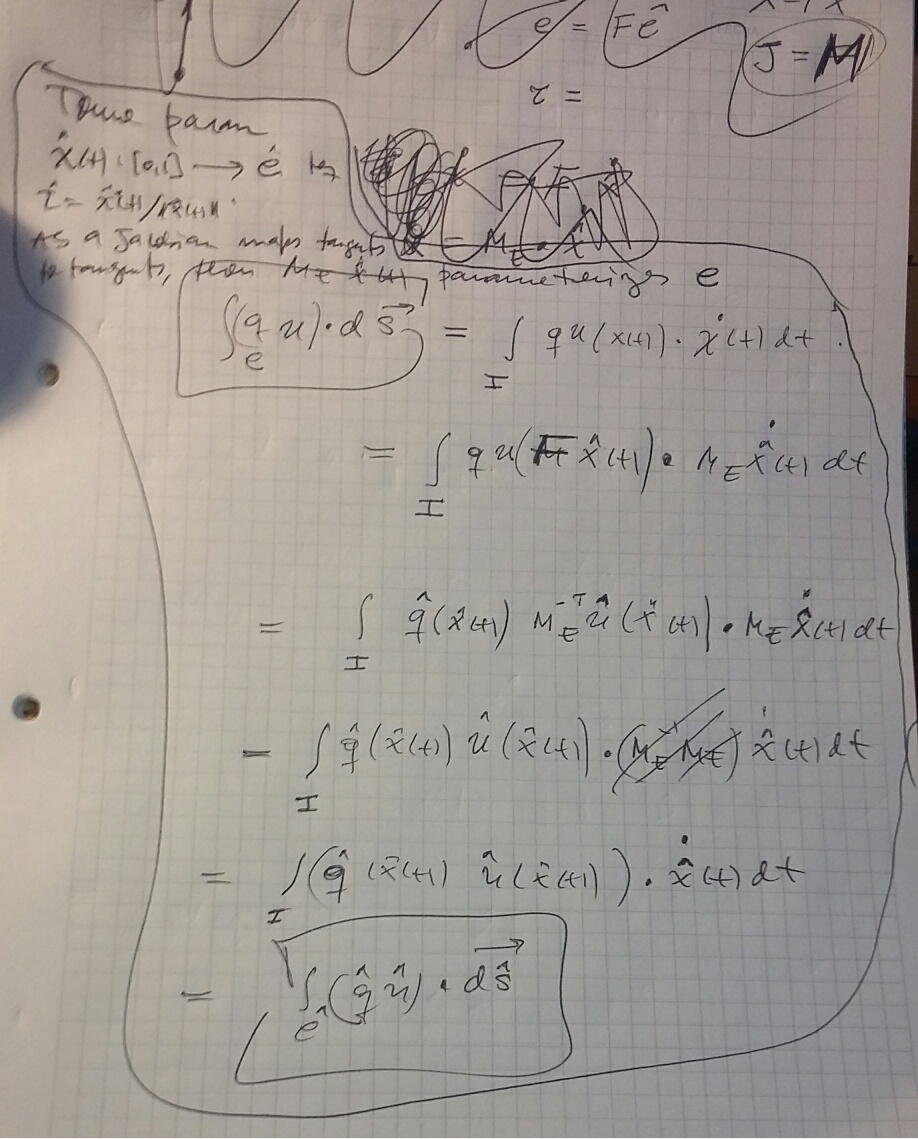
\includegraphics[scale=.15]{./figures/edgedofs.png}
  \end{figure}\\
  Face dofs: {\color{blue}\#\#\#\#\#\#\#\# continue here.}\\
  Vol dofs
  \begin{IEEEeqnarray}{rCl}
    \int_{E}\bv\cdot\br\,d\bx
    & = & 
    \int_{\hat E}M_E^{-t}\hat\bv(F_E^{-1}\bx)\cdot
      (\det M_E)^{-1}M_E\hat\br(F_E^{-1}\bx)\,d\hat\bx.\\
    & = & 
    \int_{\hat E}\hat\bv(\hat\bx)\cdot\hat\br(\hat\bx)\,d\hat\bx.
  \end{IEEEeqnarray} 
\end{proof}

\begin{lemma} The finite element in Definition~\ref{edgeelement}  is conforming
in $H\curl$ and unisolvent.
  theorem 8 page 75 in~\cite{nedelec2} is incomplete, because it is only on
  the reference element.
\end{lemma}

\begin{lemma} >Provided $\det M^{t} > 0$?, the edge element interpolators satisfy
\begin{IEEEeqnarray}{rCl}\label{piTransformado}
    \wku(\hat{\bx}) & = & M^{t} \bw_E\bu(F_E(\hat{\bx}))
\end{IEEEeqnarray}
That is, the interpolator commutes with the coordinate change~(\ref{transfHcurl}).
\end{lemma}
\begin{proof} 
\end{proof}

{\bf hcurl end}

{\bf hdiv begin}

\begin{lemma}\label{aux_label13} Let $\hat E$ be the reference prism~(\ref{defi_of_ref_prism}) and
let $P_{\hat E}$ be the space in~(\ref{prismaticSpace}).
Provided the matrix $M_E$ is block--diagonal as in Lemma~\ref{aux_label7},
then $P_{\hat{E}}$ is invariant by transformation~(\ref{transfDiv}).
\end{lemma}
\begin{proof} The proof uses the same straightforward approach as the proof of 
Lemma~\ref{aux_label7} and in a much simpler case. \noindent{\color{BrickRed}pensar esto}   
\end{proof}

\begin{lemma} \label{aux_label12}
The degrees of freedom are identical, surface and volumen integrals:
in which the faces are related by $F\hat{f} = f$.
\begin{IEEEeqnarray}{cCccl}
    \label{momentos1hdivPhys} 
    \rho_{ f,q}(\bv) & = & \int_{f} (\bv\cdot\bnu)q\,dS 
        &\quad & \mbox{for } q = \hat{q}\circ F_E^-1, \hat{q} \in P_{k-1}(\hat{f})\mbox{,}\\
    \nonumber&&&\quad&\mbox{if $ \hat{f} =  \hat{f}_3$ or $ \hat{f}_4$;}\\[5pt]
    \label{momentos2hdivPhys}
    \rho_{ f,q}(\bv) & = & \int_{f} (\bv\cdot\bnu)q\,dS 
        &\quad & \mbox{for } q = \hat{q}\circ F_E^-1, \hat{q} \in Q_{k-1, k-1}(\hat f)\mbox{,}\\
    \nonumber&&&\quad&\mbox{ if $ \hat{f} =  \hat{f}_1$, $ \hat{f}_2$ or $ \hat{f}_5$;}\\[5pt]
    \label{momentos3hdivPhys}
    \rho_{ \br}(\bv) & = & \int_{{E}} \bv\cdot\br\,d\bx 
        &\quad& \mbox{for }\br = M_E^{-t}\hat\br\circ F_E^{-1}, \hat\br\in (P_{k-2,k-1})^2 \times P_{k-1,k-2};
\end{IEEEeqnarray}
\end{lemma}
\begin{proof}
  Face dofs, by~(\ref{transfDiv}) and~(\ref{surface_diffs})
  \begin{IEEEeqnarray*}{rCl}
    \int_{f} (\bv\cdot\bnu)q\,dS & = & 
      \int_{\hat f} \hat\bv(F_E^{-1}\bx)\cdot\hat{\bnu}\frac{\hat{q}(F_E^{-1}\bx)}{\det M_E\|M_E^{-t}\hat\bnu\|}\,dS\\
      &&\int_{\hat f} (\hat\bv\cdot\hat{\boldsymbol{\nu}})\hat{q}\,d\hat{S}
  \end{IEEEeqnarray*} 
  Vol dofs
  \begin{IEEEeqnarray}{rCcCl}
    \int_{E}\bv\cdot\br\,d\bx
    & = & 
    \int_{\hat E}M_E\hat\bv\cdot M_E^{-t}\hat\br\,d\hat\bx.
    & = & 
    \int_{\hat E}\hat\bv\cdot\hat\br\,d\hat\bx.
  \end{IEEEeqnarray}
\end{proof}

\begin{lemma}
  If $\bu\in P_{E}$ is such that all the
  dofs~(\ref{momentos1hdivPhys}) or~(\ref{momentos2hdivPhys}) vanish
  on the respective face $f$, then the normal component of $\bu$ 
  vanishes identically on $f$.
\end{lemma}
\begin{proof}
  This fact is stated in the proof of Theorem 4, page $66$ of~\cite{nedelec2} 
  only for the reference prism. By transforming the degrees of freedom to 
  the faces of $\hat E$ and back to the faces of $E$ using Lemma~\ref{aux_label12}
  we get the result.
\end{proof}
\begin{lemma}
  If $\bu\in P_{E}$ is such that all the
  dofs~(\ref{momentos1hdivPhys})--(\ref{momentos3hdivPhys}) vanish, 
  then $\bu$ vanishes identically on $E$.
\end{lemma}
\begin{proof}
  In the case of the reference prism $\hat E$, we refer to the proof of 
  Theorem 4 in page $66$ of~\cite{nedelec2}.
  by the invariance of the finite element space under
  the change~(\ref{transfDiv}) (Lemma~\ref{aux_label13}) we have our result.
\end{proof}
\begin{corollary}
  Finite Element on $E$ is $H(\dv)$--conforming and unisolvent.
\end{corollary}
\begin{corollary}
  For any $\bv\in W^{1,1}(E)$ expressions 
  ~(\ref{momentos1hdivPhys})--(\ref{momentos3hdivPhys}) 
  determine a well defined local interpolate
  $\br_E\,\bu$ defined as the unique finite element function in $P_E$ such that
  \begin{IEEEeqnarray}{lClc}
    \rho_{f,\bq}\,(\bv - \br_E\,\bu) & = & 0 &
    \quad\mbox{for $\rho_{f,\bq}$ as in~(\ref{momentos1hdivPhys})
      and~(\ref{momentos2hdivPhys})}\\
    \rho_{\br}\,(\bv - \br_E\,\bu) & = & 0 &
    \quad\mbox{for $\rho_{\br}$ as in~(\ref{momentos3hdivPhys})}.
  \end{IEEEeqnarray}
\end{corollary}
And the momentos3hdivPhyswt important
\begin{corollary}
  Given $\bu \in W^{1,1}(E)$, then
  \begin{IEEEeqnarray}{rCl} \label{div_interp_commutes}
    \rku & = & \det M_E\,(M_E^{-1}\,\br_E\,\bu)\circ F_E\mbox{,}
  \end{IEEEeqnarray}
  that is, the $H(\dv)$ interpolator commutes with the coordinate
  change~(\ref{transfDiv}).
\end{corollary}

{\bf hdiv end}


\begin{remark}
  Unisolvence and conformity of the finite elements on tetrahedra in
  Section~\ref{sec:tetrahedralFEs}
  is proved in~\cite{monk}, Sections 5.4 and 5.5.
\end{remark}
%===========================
% See Lemmas 5.32 and 5.34 in pages 130 and 131 of~\cite{monk}, where
% it is proved for tetrahedra. Exacly the same considerations about the degrees
% of freedom therein apply to prove the Lemma for prisms or pyramids.  
% Ver (3.79) (3.80) en monk: transf. de normales y tangentes.\\\\
%===========================